%
% teil3.tex -- Beispiel-File für Teil 3
%
% (c) 2020 Prof Dr Andreas Müller, Hochschule Rapperswil
%
% !TEX root = ../../buch.tex
% !TEX encoding = UTF-8
%
\subsection{Evaluation
\label{genetic_algorithm:evaluation}}
Dieser Schritt befasst sich mit der auswertung der einzelnen 
Kombinationen.

In der Informatik wird die Liste genommen und die einzelnen 
zusammenstellungen ausgerechnet

Dafür wird die gleiche Fromel\ref{eq:bruteforce_min_formula}, 
wie in der Bruteforce verwendet.

\begin{figure} [h]
	\centering
	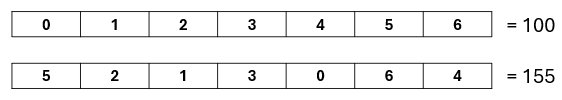
\includegraphics[width=0.8\textwidth]{
        papers/variationsprinzip_algorithmen/images/teil2/03_genetic_string_cities_results.png
        }
	\caption{Beispiel von genetischen String mit Resultate}
	\label{fig:cities_genetic_string_results}
\end{figure}

